Tečky
40 %

%TEXT%
Na bílém papíře je do čtverce zakresleno devět teček. Vaším úkolem je nakreslit
do obrázku čtyři úsečky tak, aby procházeli všemi devíti tečkami. Čáry musíte
nakreslit jedním tahem - nesmíte zvednou pero z~papíru.

\begin{center}
	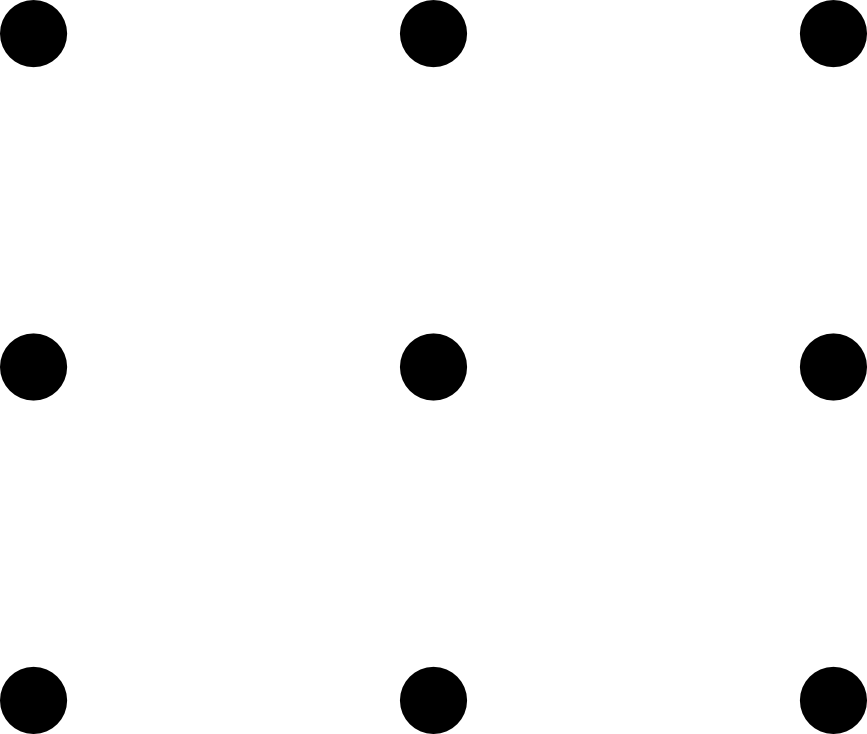
\includegraphics[width=0.3\textwidth]{../data/Rychlovky/tecky.png}
\end{center}
~

%BAD%
Úsečky jsou úsečky, žádné křivky.

%HELP%
Jako obvykle se musíte dostat za rámec svého uvažování.

%SOLUTION%
\begin{center}
	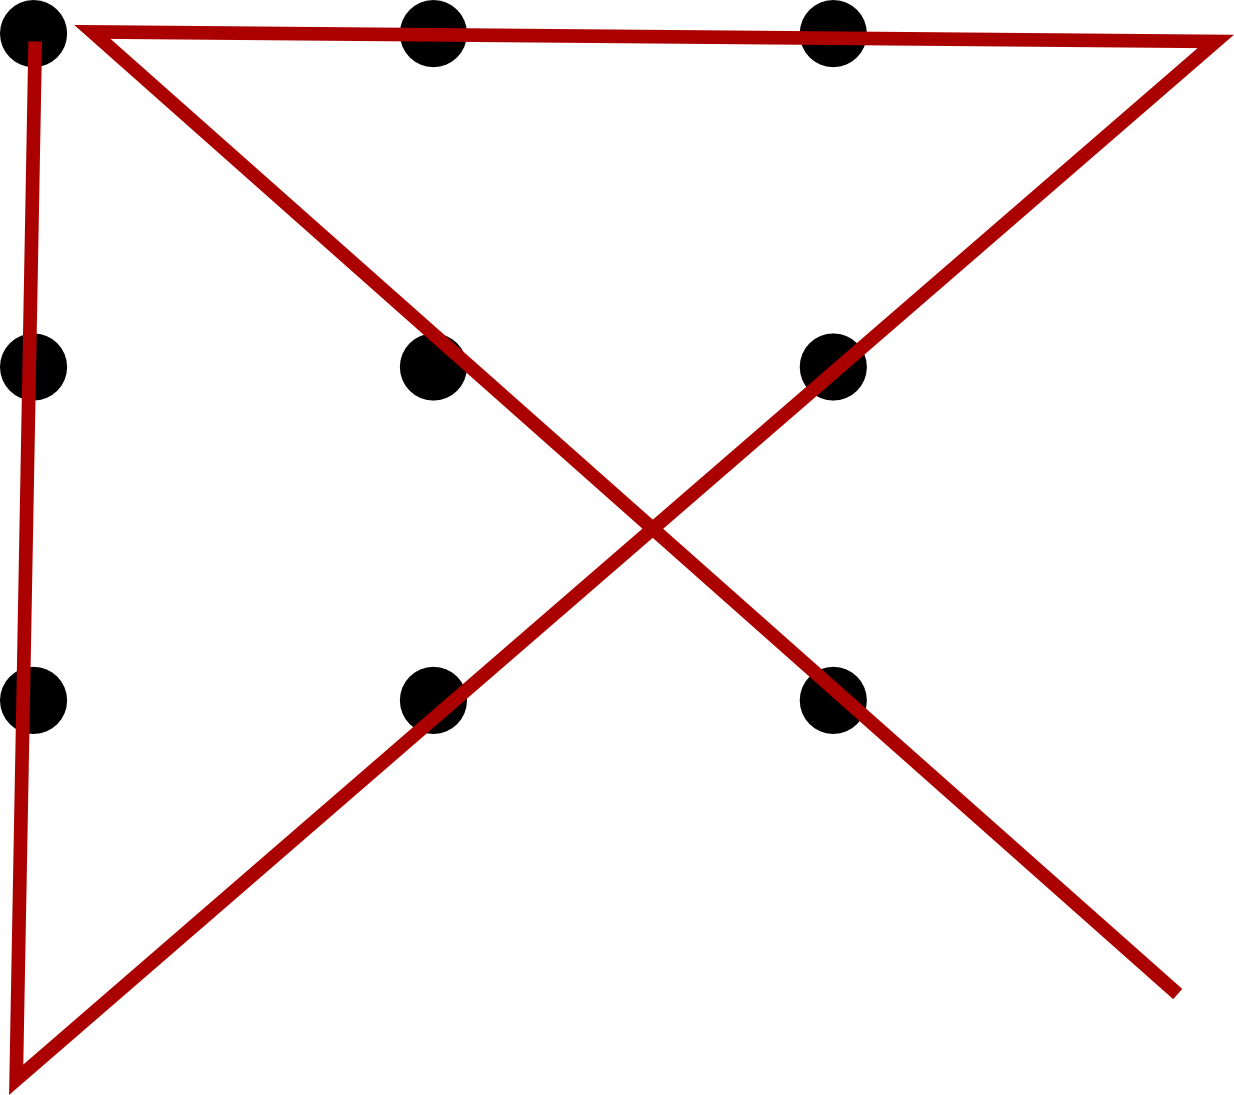
\includegraphics[width=0.3\textwidth]{../data/Rychlovky/tecky_reseni.png}
\end{center}
